\documentclass[11pt, margin=1in]{article}
\usepackage{amsmath}
\usepackage{amsfonts}
\usepackage{amssymb}
\usepackage[margin=1in]{geometry}
\usepackage{fancyhdr}
\usepackage{natbib}
\usepackage{hyperref}
\usepackage{booktabs} % Top and bottom rules for tables


\hypersetup{
    colorlinks=true,
    citecolor=blue,
    urlcolor=red
}

% Use these for theorems, lemmas, proofs, etc.
\newtheorem{theorem}{Theorem}
\newtheorem{lemma}[theorem]{Lemma}
\newtheorem{proposition}[theorem]{Proposition}
\newtheorem{claim}[theorem]{Claim}
\newtheorem{corollary}[theorem]{Corollary}
\newtheorem{definition}[theorem]{Definition}
\newtheorem{fact}[theorem]{Fact}
\usepackage{tikz}
\usetikzlibrary{arrows}
\newenvironment{proof}{\noindent {\it Proof.}}{\hfill\rule{2mm}{2mm}}
\pagestyle{fancy}
\lhead{\textbf{CS236r Final Report}}
\rhead{\textit{Alex Lin \& Melissa Yu}}
\cfoot{\thepage}
\renewcommand{\headrulewidth}{0.4pt}
\renewcommand{\footrulewidth}{0.4pt}
\newcommand{\card}[1]{\ensuremath{\left\vert#1\right\vert}}
\newcommand{\diff}[1]{\, d#1}
\newcommand{\eval}[2]{\Big|_{#1}^{#2}}
\newcommand{\vect}[1]{\boldsymbol{#1}}
\newcommand{\R}{\mathbb{R}}
\newcommand{\E}{\mathbb{E}}
\newcommand{\norm}[1]{\left\lVert#1\right\rVert}

\makeatletter

\begin{document}
	
\title{CS236r Final Report \\ Fair and Interpretable Models for Credit Scoring}
\author{Alex Lin \and Melissa Yu}
\date{}
\maketitle

\begin{abstract}
Credit scoring models are widely used to separate consumers into one of two groups -- "good" customers who are likely to repay their debt and "bad" customers who are likely to default on loans.  Since theses models have such a significant impact on financial opportunities in everyday life -- from buying a house to getting a job to starting a business -- it is imperative that they are accurate, fair, and interpretable.  Off-the-shelf, black-box algorithms such as neural networks can be very accurate, yet are not easy to interpret and are prone to producing unfair results, especially when trained on historically unjust data.  In combining the RiskSLIM algorithm \cite{risk-slim} with constraints for reducing disparate impact \cite{disparate-impact}, we create fair scoring rules that are easy to understand and also compliant with the Equal Credit Opportunity Act.  We additionally explore the accuracy vs. fairness/interpretability tradeoff in greater detail, showing how we can satisfy constraints on the latter without giving up too much of the former. \\ \\  
\textbf{Keywords:} credit scoring, scoring rules, disparate impact, neural networks, accuracy, fairness, interpretability
\end{abstract}

\section{Introduction}
Consumer spending is among the most important determinants of macroeconomic conditions and systemic risk, accounting for around 70\% of the U.S. GDP between 2001 and 2010 \cite{ml-for-risk}. As the credit industry has rapidly expanded over the last few decades, the risk associated with consumer lending has multiplied as well. Today, it is more important than ever that financial institutions leverage accurate, interpretable prediction models and algorithms to make the many lending decisions they must process on a daily basis, instead of relying on potentially biased, inaccurate, and un-scalable human discretion. These predictive algorithms leverage characteristics pulled from the consumer credit files collected by credit bureau agencies to discern the riskiness of a loan.

\textit{Credit scoring models} are quantitative models widely used by financial institutions to determine the probability of delinquency or default for loan applicants \cite{nn-scoring-models}. These models have as their goal accurately classifying loan applicants into one of two groups: ``good'' customers, who are likely to repay their debt, and ``bad'' customers, who are denied credit on the basis that they are likely to default.

In order for lenders to leverage scoring algorithms to make smart lending decisions, the model they use must satisfy several requirements \cite{fico-criteria}:
\begin{enumerate}
	\item \textbf{Predictive power}: The model should make accurate predictions of customer type -- good or bad.
	\item \textbf{Fairness}: The model must comply with the Equal Credit Opportunity Act (ECOA) and Fair Credit Reporting Act (FCRA). It cannot discriminate on the basis of race, age, education, employment history, gender, marital status, or wealth.
	\item \textbf{Broad coverage}: The model is adaptable enough to apply across large datasets of people.
	\item \textbf{Data transparency}: The data used in the model is verifiable and correctable by consumers.
	\item \textbf{Interpretability (consumer-focused)}: The model's classification process can be easily explained to and understood by consumers, and the most important predictive factors can be intuitively identified to aid loan seekers in improving their profile.
\end{enumerate}

Many off-the-shelf, black-box machine learning algorithms are heavily (and perhaps overly) concerned with requirement (1) listed above.  There exist all sorts of tips and tricks for increasing a model's predictive power, including cross-validation, weight regularization, ensemble methods, and many more \cite{ml-review}.  Optimizing predictive accuracy is arguably the main focus of machine learning.  In addition, by using large, publicly available datasets, machine learning engineers can often satisfy requirements (3) and (4) in an easy manner.  

However, the machine learning community has not traditionally paid much attention towards metrics such as fairness and interpretability.  Yet, these metrics are very important in high-risk settings such as the credit scoring problem.  Due to historical injustices against currently protected subgroups of the population, it may be neither reasonable nor fair to naively train a model on biased data.  Furthermore, although complicated models such as neural networks and random forests can serve as very accurate classifiers, they can often be difficult for the average consumer to understand \cite{nn-interpretable}.  It may be challenging for someone without the requisite mathematical background to identify which features of the model they should target in order to improve their own credit score.  

In this paper, we aim to create models for credit scoring that are both fair and interpretable.  The specific type of model we will use is called a \emph{scoring rule}.  In Section 2, we argue that scoring rules are clearly more interpretable than other potential model choices.  Scoring rules can be generated using Ustun and Rudin's RiskSLIM algorithm, a procedure that formulates the problem of finding coefficients for scoring rules as a Mixed Integer Nonlinear Program (MINLP) \cite{risk-slim}.  Section 3 focuses on fairness and specifically, how we can combine RiskSLIM with constraints for reducing \emph{disparate impact}, as formulated by Zafar et. al \cite{disparate-impact}.  In Section 4, we give an overview of the \href{https://archive.ics.uci.edu/ml/datasets/statlog+(german+credit+data)}{German Credit Data Set} that we use for model development.  We also introduce a baseline neural network as well as our methods for applying RiskSLIM to create fair and interpretable scoring rules.  Section 5 presents results and an analysis of the tradeoff between accuracy vs. fairness and interpretability for these scoring rules.  Finally, Section 6 concludes the paper with a brief discussion and a few ideas for future work.    

\section{Increasing Interpretability: Scoring Rules}

Scoring systems are linear classification models that only require users to add, subtract and multiply a few small numbers in order to make a prediction \cite{slim}.  This makes them remarkably easy to understand for the average layman, especially when compared to other machine learning models used for prediction.  

\subsection{Scoring Rules for High-Risk Problems}
When working in high-risk settings such as credit scoring, it is imperative that users feel that they can interpret the models that are available to them.  If they see an algorithm as nothing more than a black-box, then there is a good chance that they will inherently mistrust its capabilities.  

This is exactly why scoring systems may be desirable for high-risk problems in domains such as medicine and law \cite{slim, risk-slim} in which the cost of a misclassification can have grave consequences.  Using classical optimization techniques in Mixed Integer Programming (MIP), Ustun and Rudin were able to develop an algorithm called the Supersparse Linear Integer Model (SLIM) that can generate generic scoring systems while taking into account factors such as algorithmic fairness and interpretable coefficients \cite{slim}.  Although SLIM produces simple models, its models also seem to exhibit high accuracy under AUC measures.  The authors further developed RiskSLIM, which can produce scoring systems that not only make a prediction, but can also incorporate risk assessment into that prediction \cite{risk-slim}.  In other words, each score outputted by RiskSLIM scoring rules will be correlated with the probability of falling in the positive class.  Figure 1 gives an example of a risk-calibrated scoring rule for predicting stroke.  

\begin{figure}
\begin{center}
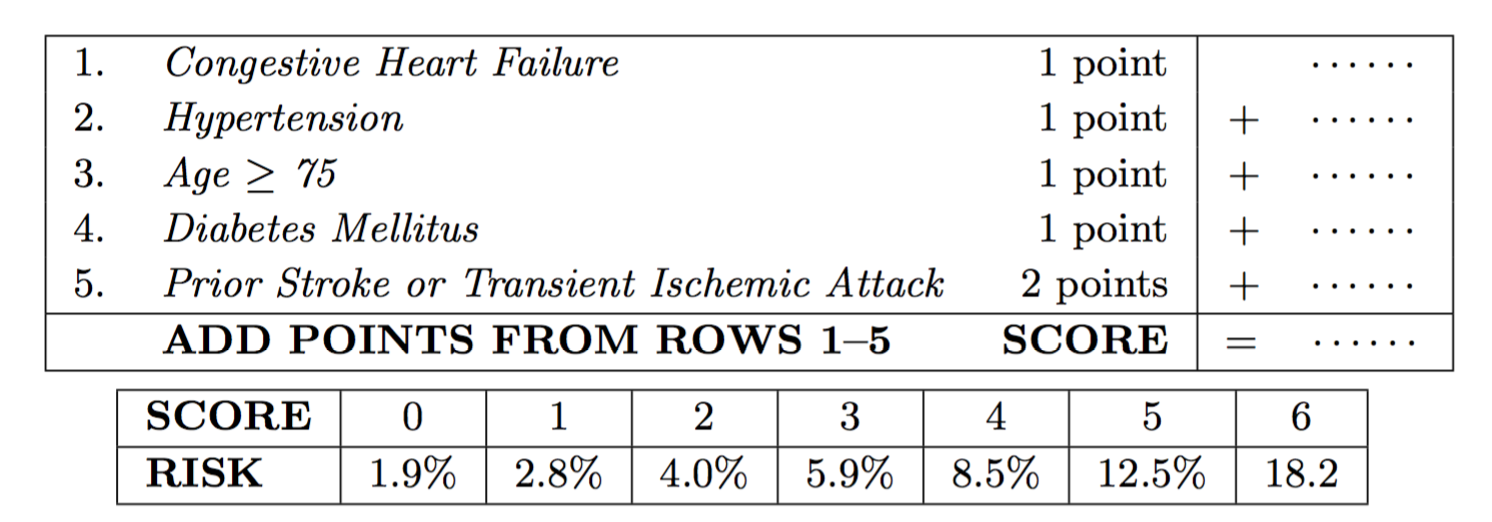
\includegraphics[scale=0.5]{img/scoring-rule}
\end{center}
\caption{Risk-calibrated scoring rule for assessing stroke risk \cite{stroke}.}
\end{figure}

\subsection{RiskSLIM Algorithm}

Our models for credit scoring will employ the RiskSLIM algorithm, because we want the scores to be risk-calibrated.  We argue that risk-calibrated scores increase interpretability for the average layman, since it tells people that they should try to decrease their score in order to decrease their risk of being a "bad" consumer and improve their credit rating.   

The RiskSLIM Algorithm works as follows: Let there be $N$ training examples where each example $i \in 1, \ldots, N$ has an associated feature vector $\vect{x}_i = [x_1, \ldots, x_d]^T$ and a response variable $y_i \in \{1, -1\}$, where $1$ corresponds to a good consumer and $-1$ corresponds to a bad consumer.  The RiskSLIM algorithm essentially solves a Mixed Integer Non-Linear Program (MINLP) to find a vector of coefficients $\vect{\lambda} = [\lambda_1, \ldots, \lambda_d]^T$ and a bias term $\lambda_0$ such that the probability of being a bad customer is
\begin{align*}
p(y_i = 1 \vert \vect{x}_i) = \frac{1}{1 + \exp(- \vect{\lambda} \cdot \vect{x}_i - \lambda_0)}
\end{align*}
where $\cdot$ denotes the dot product between the two vectors.  A standard logistic regression classifier satisfies the formulation described above while optimizing for \emph{risk calibration accuracy}, which is defined as minimizing the cross-entropy loss $l(\vect{\lambda}, \lambda_0)$ between the data's true distribution and the distribution that the model attributes to the data:
\begin{align*}
l(\vect{\lambda}, \lambda_0) = \sum_{i=1}^N y_i \cdot \log p(y_i = 1 \vert \vect{x}_i) + (1 - y_i) \cdot \log (1 - p(y_i = 1 \vert \vect{x}_i)) 
\end{align*}     
The RiskSLIM MINLP formulation adds at least two other constraints to this standard logistic regression formulation.  

First, we want to ensure that the coefficients are sparse; that is, scoring rules only want a few of them to be nonzero.  This minimization is expressed by adding the term $C_0 \norm{\vect{\lambda}}_0$ to the objective function, where $C_0$ is a constant that controls the tradeoff.    

Second, we want the coefficients to be small integers.  Thus, we add constraints restricting $\vect{\lambda} \in \{-5, \ldots, 5\}^d$ and $\lambda_0 \in \{-5, ,\ldots, 5\}$.  The full MINLP formulation is given below: 
\begin{align*}
&\min_{\vect{\lambda}, \lambda_0} \quad l(\vect{\lambda}, \lambda_0) + C_0 \norm{\vect{\lambda}}_0 \\
&\text{s.t.} \quad \vect{\lambda} \in \{-5, \ldots, 5\}^d \\
&\quad \quad \lambda_0 \in \{-5, \ldots, 5\}
\end{align*}       

Using a lattice place cutting algorithm, Ustun and Rudin devise a clever branch-and-bound method to solve this MINLP.  The essential idea is to alternate between steps to reduce the optimality gap and steps for discovering new feasible solutions.  See \cite{risk-slim} for additional details.  The output of their algorithm is optimal coefficients $\vect{\lambda}, \lambda_0$ that can be used to create scoring rules.  

\section{Increasing Fairness: Constraining Disparate Impact}

Although the RiskSLIM algorithm can produce models that increase interpretability, there are no guarantees about fairness.  If trained on a historically unfair dataset, the scoring rules that are produced will be unfair as well.  In fact, Ustun and Rudin note at the end of their RiskSLIM paper that "one interesting direction for future work includes using our proposed approach to build risk scores with constraints to enforce fairness" \cite{risk-slim}.  We explore this direction in our paper.  

\subsection{Disparate Impact}
Disparate impact is the notion in which a model's biased classification process leads to outcomes that disproportionately hurt (or benefit) people with sensitive attributes.  In the credit scoring example, we define "sensitive attributes" as those that are listed under ECOA and FCRA.  Specifically, these are race, age, education, employment history, gender, marital status, and wealth.  

As an example, if historical data is sexist towards females and the probability of being a "good" customer is negatively correlated with being female, then a model trained on this data may also be more likely to classify females as "bad" customers.  Any bank using such a model to approve loan requests could end up denying consumers on the basis that they are female -- which is clearly unfair.  In order to avoid this disparate impact, we follow Zafar et. al in formalizing fairness constraints \cite{disparate-impact}.  

Note that we chose to focus on disparate impact instead of disparate mistreatment \cite{disparate-mistreatment} because we assume that we do not have "ground truth" training data; that is, due to historical injustices, we cannot necessarily trust our credit scoring dataset to be unbiased and 100\% reflective of the true "good" vs. "bad" distribution of consumers.   

\subsection{Decision Boundary Covariance for Fairness Constraints}    
Zafar et. al \cite{disparate-impact} use the following method to constrain logistic regression problems in a more fair setting:  Assume that the feature vectors $\vect{x}_1, \ldots, \vect{x}_N$ do not contain sensitive attributes.  Let example $i$'s sensitive attributes (latent to the classifier) be denoted $\vect{z}_i$.  To simplify things, we will assume for the rest of this paper that each $z_i \in \vect{z}_i$ is binary.  

Note that the model can still produce unfair classifications even if $\vect{z}$ is never seen directly, because there may be an observed feature $x \in \vect{x}$ that is correlated with $\vect{z}$.

The $p$\% rule captures the essence of fighting disparate impact.  It states that for a given $p \in \{0, \ldots 100\}$ and some $z \in \vect{z}$, we should constrain the ratio of those in the positive class given $z = 1$ vs. those in the positive class given $z = 0$ to be at least $p / 100$.  When working with linear decision boundaries defined by some weight vector $\vect{\lambda}$ and some bias $\lambda_0$ (such as in logistic regression and scoring rules), classifying example $i$ as being in the positive class is simply the same as having $\vect{\lambda} \cdot \vect{x}_i + \lambda_0 \geq 0$.  Thus, the $p$\% rule requires
\begin{align*}
\frac{p(\vect{\lambda} \cdot \vect{x} + \lambda_0 \geq 0 \vert z = 1)}{p(\vect{\lambda} \cdot \vect{x} + \lambda_0 \geq 0 \vert z = 0)} > \frac{p}{100}  & & \frac{p(\vect{\lambda} \cdot \vect{x} + \lambda_0 \geq 0 \vert z = 0)}{p(\vect{\lambda} \cdot \vect{x} + \lambda_0 \geq 0 \vert z = 1)} > \frac{p}{100}
\end{align*}  
This constraint is a non-convex function of $\vect{\lambda}, \lambda_0$, so instead, Zafar et. al turn to constraints on the covariance between $\vect{z}$ and the distance to the decision boundary $d_{\vect{\lambda}, \lambda_0}(\vect{x}) =  \vect{\lambda} \cdot \vect{x} + \lambda_0$ \cite{disparate-impact}.  Intuitively, if this covariance is 0, then knowing $\vect{z}$ should have no impact on knowing $p(y \vert \vect{x})$, which is the definition of having zero disparate impact.  We can empirically evaluate this covariance as 
\begin{align*}
\mathbb{C}\text{ov}(\vect{z}, d_{\vect{\lambda}, \lambda_0}(\vect{x})) &= \E[(\vect{z} - \vect{\bar{z}})(d_{\vect{\lambda}, \lambda_0}(\vect{x}) - \bar{d}_{\vect{\lambda}, \lambda_0}(\vect{x}))] \\
&= \E[(\vect{z} - \vect{\bar{z}}) \times d_{\vect{\lambda}, \lambda_0}(\vect{x})] - \E[(\vect{z} - \vect{\bar{z}})]  \times \bar{d}_{\vect{\lambda}, \lambda_0}(\vect{x}) \\
&= \E[(\vect{z} - \vect{\bar{z}}) \times d_{\vect{\lambda}, \lambda_0}(\vect{x})] \\
&\approx \frac{1}{N}\sum_{i=1}^N (\vect{z}_i - \vect{\bar{z}}) \times d_{\vect{\lambda}, \lambda_0}(\vect{x}_i)
\end{align*}
where $\vect{\bar{z}} \approx \frac{1}{N} \sum_{i=1}^N \vect{z}_i$.  Note that putting a constraint on this final quantity to be less than or equal to some $\vect{c}$ is certainly a linear constraint on $\vect{\lambda}, \lambda_0$.  To correct for disparate impact, we will enforce such a relationship, as explained below.  

\subsection{Reformulating RiskSLIM}

To account for fairness along with interpretability, we reformulate the RiskSLIM with the aforementioned disparate impact constraint:   
\begin{align*}
&\min_{\vect{\lambda}, \lambda_0} \quad l(\vect{\lambda}, \lambda_0) + C_0 \norm{\vect{\lambda}}_0 \\
&\text{s.t.} \quad \vect{\lambda} \in \{-5, \ldots, 5\}^d \\
&\quad \quad \lambda_0 \in \{-5, \ldots, 5\} \\
& \quad \quad \frac{1}{N}\sum_{i=1}^N (\vect{z}_i - \vect{\bar{z}}) \times (\vect{\lambda} \cdot \vect{x}_i + \lambda_0) \leq \vect{c} \\
& \quad \quad \frac{1}{N}\sum_{i=1}^N (\vect{z}_i - \vect{\bar{z}}) \times (\vect{\lambda} \cdot \vect{x}_i + \lambda_0) \geq -\vect{c}
\end{align*}
for some inputted hyper-parameters $C_0$ and $\vect{c}$.           

%----------------------------------------------------------------------------------------
%	METHODS
%----------------------------------------------------------------------------------------

\section{Methods} \label{sec:methods}

\subsection{Data} \label{ssec:data}

Following the convention of previous work in the field, we use the German credit (GC) dataset from the UCI Library \cite{data}, which contains 1000 historical credit cases. Each case is labeled by a binary response variable, which indicates whether the customer is ``bad,'' along with 7 numerical and 13 categorical features. These covariates capture information from both loan application forms (e.g., loan amount, interest rate, purpose, duration) and customer information (e.g., demographic, socioeconomic, and past solvency data). 

Among the original 20 features, we identify 3 in accordance with the ECOA and FCRA as sensitive attributes which we would like to maintain fairness with respect to: \texttt{age}, \texttt{sex}, and \texttt{maritalStatus}. For simplicity and tractability, we encode each of these features as a binary indicator variable. Specifically, \texttt{age} is transformed into the indicator of being over age 35, \texttt{sex} is converted to the indicator of being male, and  \texttt{maritalStatus} becomes the indicator of \textit{not} being single. All remaining categorical features are one-hot encoded. After preprocessing, each data point has 58 features, including the 3 sensitive ones. 

Of the 1000 loans included in the dataset, 300 are labeled as ``bad,'' or defaulted, giving a prior default rate of 0.3. Although class imbalance can impact classifier performance, we do not correct this relatively moderate  imbalance through re-sampling. This decision is based on our primary objective, which is to compare the relative performance differences between several classifiers and our proposed model. Re-sampling is also unlikely in corporate practice. Using the data as-is allows us to more closely simulate the real use of such an algorithm. 

\subsection{Baseline} \label{ssec:baseline}

We make a distinction between \textit{individual classifiers } (e.g., CART, Linear support vector machine, Logistic Regression, Multilayer perceptron artificial neural network) and \textit{ensemble methods}, which pool predictions from many classification models (e.g, Bagged decision trees, Simple average ensemble). Because RiskSLIM is an individual classifier, we choose to compare our proposed model with an individual baseline. Multilayer perceptron artificial neural networks (ANNs) have recently been shown to achieve the best overall performance among many other individual classifiers in credit scoring applications \cite{benchmarks}. We implement an ANN as our baseline model.

Given their demonstrated performance in this task, we expect ANN's to have good predictive power. However, even a single layer neural network is highly uninterpretable: Common methods of interpreting or explaining the output of a neural network include examining the learned weights, or tweaking singular input features to observe the effect of such a change on the output. Ultimately, the model's classification process is a black box that cannot be easily explained to or understood by consumers. Moreover, the most important predictive factors cannot be easily and intuitively identified to aid loan seekers in improving their profile. 

\subsection{Model}

We enforce disparate treatment by excluding the sensitive attributes from the set of predictors fed into all models. We enforce disparate impact by adding the following set of linear constraints for each sensitive attribute $z$:
\begin{align*}
\frac{1}{N} \sum_{i=1}^N (z_i - \bar{z}) \times (\vect{\lambda} \cdot \vect{x}_i + \lambda_0) &\leq c_z\\
\frac{1}{N} \sum_{i=1}^N (z_i - \bar{z}) \times (\vect{\lambda} \cdot \vect{x}_i + \lambda_0) &\geq -c_z 
\end{align*}
where $z \in \{age, sex, maritalStatus\}$ in our case.

\subsection{Implementation}

We formulate an instance of the RiskSlimMINLP with the constraints: $\lambda_0 \in \{-50, \dots, 50\}$, $\lambda_j \in \{-5, \dots, 5\}$ for $j > 0$, and $\vert\vert\vect{\lambda}\vert\vert_0\leq 5$. We set the penalty parameter $C_0=10^{-6}$ so that the optimizer of RiskSlimMINLP belongs to the $C_0$-level set of feasible models and cap runtime at 1,500 seconds (25 minutes).

Our constrained RiskSLIM model is implemented on top of the Python / CPLEX software for RiskSLIM computing \href{https://github.com/ustunb/risk-slim}{published by the authors}, and adapt their script for our use by adding CPLEX linear constraints as described in the previous section. We use PyTorch to implement the baseline, a single-layer, linear, feedforward neural net with hidden layer size 50 and ReLU activations. The model was trained using the Adam optimizer with learning rate 0.0001 over 100 epochs. 

\subsection{Evaluation}

Following \cite{risk-slim}, we benchmark the performance of our models in terms of \textit{Rank Accuracy}, evaluated as area under the ROC curve (AUC). A model with high rank accuracy outputs risk scores that can be used to order examples in terms of their true risk, an important property for credit scoring models. We additionally assess the fairness of our classifiers (disparate impact) by calculating the ``$p$\%-rule'' corresponding to its decision boundary for each sensitive attribute. Higher values of $p$ indicate greater fairness in this framework.

%----------------------------------------------------------------------------------------
%	RESULTS
%----------------------------------------------------------------------------------------

\section{Results} \label{sec:results}

We find that enforcing fairness constraints across all 3 sensitive attributes simultaneously is quite computationally restrictive, leading the model to find solutions with very low AUCs in order to satisfy all the constraints with very high computation times. As a result, we focus on single-constraint models in this section, where only one of the sensitive attributes is restricted at a time.

Table 1 shows the best performance achieved by our classifiers in terms of AUC and the $p$\%-rule for each sensitive attribute. As expected, the AUC is highest for the ANN model. However, this model has very low fairness, satisfying $p$\%-rules of only around 20\% for each sensitive attribute. In contrast, the constrained RiskSLIM models have AUCs that are lower than the ANN by around 10\% each, but boast much higher values for $p$. Notably, we see that the optimal (highest) value for $p$ for each sensitive attribute is obtained using the model with an explicit constraint on that attribute's disparate impact, indicating that our constraints have done their job well. Although we only constrained one sensitive attribute at a time, we note that the $p$\% thresholds for all attributes were consistently greater than 80\%, indicating that simultaneously constraining all three attributes may be unnecessary. The unconstrained RiskSLIM classifier has a higher average AUC, and $p$ rules around 30\%, further showing that our rules have substantially increased the performance of the classifier.

Figure 2 shows a set of sample scoring constrained RiskSLIM models. The features identified by our algorithm are easily explainable and justifiable to consumers, and many of them are already understood as common knowledge. These scoring models enable consumers and providers to quickly identify the most important predictive factors (by examining the relative weights assigned to each of less than 5 features), and thus allow us to transparently aid loan seekers in improving their profile.

We additionally visualize the tradeoff between a classifier's AUC score and its fairness for varying values of the parameter $c_z$ in Figure 3. As expected, the AUC score increases as $c_z$ increases, while the fairness decreases.

\begin{table*} \label{table:baselines}
	\centering
	\begin{tabular}{lcccc}
		\toprule
		Classifier & AUC & $p_{age}$ & $p_{sex}$ & $p_{marital}$\\
		\midrule
		ANN & \textbf{0.8075} & 0.1774 & 0.1792 & 0.2950 \\
		RiskSLIM (unconstrained) & 0.7365 & 0.3495 & 0.3957 & 0.3797 \\
		RiskSLIM + age & 0.7204 & \textbf{0.9791} & 0.8948 & 0.9339 \\
		RiskSLIM + sex & 0.7053 & 0.9432 & \textbf{0.9614} & 0.9251 \\
		RiskSLIM + maritalStatus & 0.7075 & 0.9202 & 0.9376 & \textbf{0.9679} \\
		\bottomrule
	\end{tabular}
	\caption{Baseline binary classification performance on the German Credit dataset \cite{data}. Our RiskSLIM results are averaged over 5 full runs of the algorithm each. The best result for each metric is highlighted in bold.}
	\label{fig:baselines}
\end{table*}

\begin{figure*} \label{fig:samples}
	\centering
	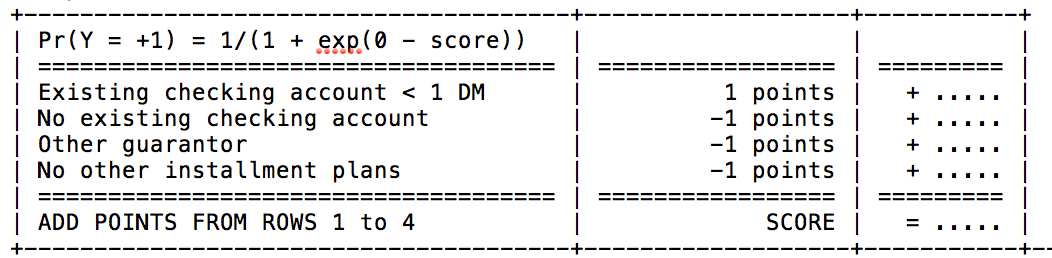
\includegraphics[width=0.7\linewidth]{img/sample1}
	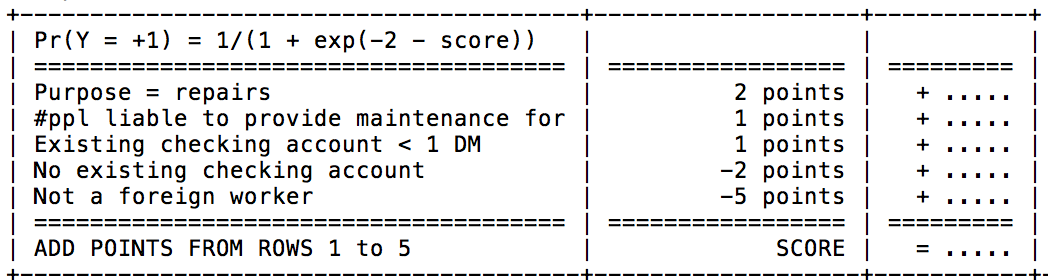
\includegraphics[width=0.7\linewidth]{img/sample2}
	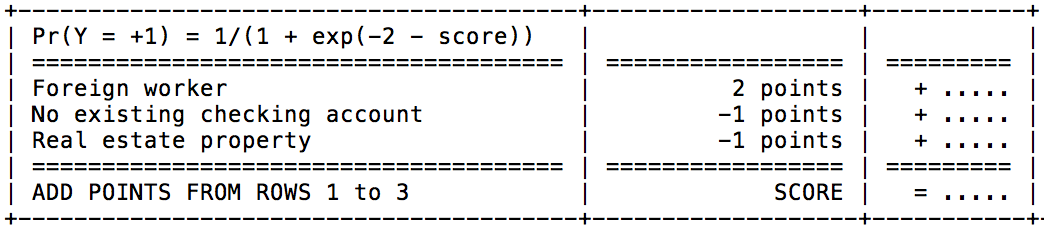
\includegraphics[width=0.7\linewidth]{img/sample3}
	\caption{Sample models generated by the age- (top), sex- (middle), and marital status- (bottom) constrained RiskSLIM algorithm. Lower scores indicate lower default risk.}
\end{figure*}

\begin{figure*} \label{fig:tradeoffs}
	\centering
	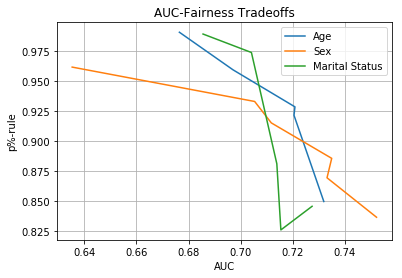
\includegraphics[width=0.7\linewidth]{img/tradeoffs}
	\caption{Tradeoff between model AUC score and fairness for constrained RiskSLIM models. Each data point comes from 5 averaged runs of the algorithm for a set $c$.}
\end{figure*}

\section{Conclusion}
This paper presented a fair credit scoring classification model built on the RiskSLIM risk scoring method. We showed that the resulting models are both highly interpretable, with at most 5 features used in a linear combination, and quite fair, with respect to the disparate impact measure, while still maintaining relatively competitive rank accuracies compared to a benchmark neural network. Future work includes further exploring fully constrained RiskSLIM formulations, where all sensitive attribute constraints can be simultaneously enforced.  Such work may require us to reform parts of the RiskSLIM lattice cutting plane algorithm in order to speed up run time.   

\bibliographystyle{abbrv}
\bibliography{refs}

\end{document}